\documentclass[a4paper,12pt,titlepage,floatssmall,abstract=off]{article}

% Page geometry's formatting
\usepackage[left=2.5cm,right=2.5cm,top=2.5cm,bottom=2.5cm]{geometry}
\usepackage{indentfirst}
\usepackage{placeins}
\usepackage{float}
% Language-specific settings
\usepackage[T1]{fontenc}
\usepackage[utf8]{inputenc}
\usepackage[polish]{babel}
\usepackage{polski}
% Elements' embedding
\usepackage{listings}
\usepackage{graphicx}
\usepackage{hyperref}
% Text-formatting
\usepackage[dvipsnames]{xcolor}
\usepackage[autostyle]{csquotes}
\usepackage{moresize}
\usepackage{amsmath}
% Miscellaneous
\usepackage[backend=biber,style=ieee]{biblatex}
\usepackage[enable]{easy-todo}
\usepackage{lipsum}

% ============================================================================================================== %
% ----------------------------------------------- Configuration ------------------------------------------------ %
% ============================================================================================================== %

% Bibliography file
\addbibresource{tex/bibliography.bib}

% Unordered list
\renewcommand{\labelitemi}{\textbullet}

% Removing clearpage after abstract
\makeatletter
\renewenvironment{abstract}{%
      %\titlepage
      %\null\vfil
      \@beginparpenalty\@lowpenalty
      \small
      \begin{center}%
        \bfseries \abstractname
        \@endparpenalty\@M
      \end{center}\quotation}%
     {\quotation\par%\vfil\null\endtitlepage
     }
\makeatother

% Listings formatting
\lstdefinestyle{customc}{
  belowcaptionskip=1\baselineskip,
  breaklines=true,
  frame=L,
  xleftmargin=\parindent,
  language=C,
  showstringspaces=false,
  basicstyle=\footnotesize\ttfamily,
  keywordstyle=\bfseries\color{purple},
  commentstyle=\itshape\color{ForestGreen},
  identifierstyle=\color{blue},
  stringstyle=\color{orange},
}

% ============================================================================================================== %
% --------------------------------------------- Macrodefinitions ----------------------------------------------- %
% ============================================================================================================== %

% Redefininiton of the title page
\renewcommand{\maketitle}{
\begin{titlepage}
    \vfill
    \begin{center}
        \begin{figure}
            \centering
            
\includegraphics[scale=0.9]{img/header.png}
            \vspace{0.5cm}
        \end{figure}
    \end{center}
    \vspace{2cm}
    \begin{center}
        {\HUGE {\bf Obiekty Internetu Rzeczy}}\\
        \vspace {0.4cm}
        {\Large {(projekt)}}
    \end{center}
    \vspace{4cm}
    \begin{center}
        {\bf \LARGE Aplikacji węzła Internetu Rzeczy \\z~interfejsem CoAP}
        \vspace{3cm}
    \end{center}
    \vfill
    \begin{center}
        {\bf \normalsize Pierczyk Krzysztof, Troć Patryk}
    \end{center}
    \vfill
    \begin{center}
        \large{Warszawa, \today \par}
    \end{center}
\end{titlepage}
}


% ============================================================================================================== %
% --------------------------------------------------- Text ----------------------------------------------------- %
% ============================================================================================================== %

\begin{document}

% Title
\maketitle

% Table of content
\tableofcontents
\clearpage

% Chapters
\section{Wstęp}

Celem projektu było stworzenie aplikacji serwerowej dla obiektu Internetu Rzeczy działającej w~oparciu o~autorską lub dostępną publicznie implementację protokołu CoAP (ang. \textit{Constrained Application Protocol}). Platformą docelową został moduł \mbox{\textbf{NodeMCU}} w~wersji trzeciej wyposarzony w~układ SoC ESP8266 oraz 4MiB pamięci Flash dołączonej za pośrednictwem interfejsu Quad SPI. Niewątpliwą zaletą urządzenia jest zintegrowany moduł WiFi w~standardzie 802.11b/g/n. Na płytce umieszczony został układ CH340 umożliwiający komunikację z~wykorzystaniem protokołu USB $\leftrightarrow$ UART.

\begin{figure}[h]
    \centering
    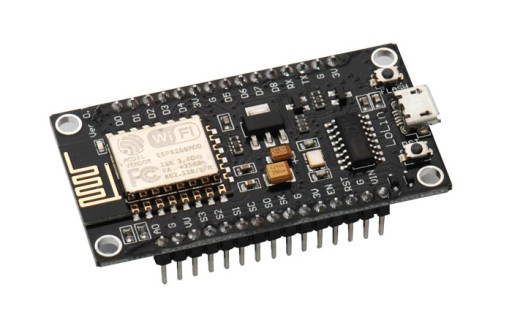
\includegraphics[scale=0.6]{img/esp8266.jpg}
    \label{esp8266}
    \caption{Płytka rozwojowa NodeMCU w~wersjii trzeciej}
\end{figure}
\vspace{0.5cm}

Istnieją dwie zasadnicze możliwości programowania układów z~rodziny ESP. Pierwsza z~nich to dostosowany do możliwości platformy interfejs Arduino. Dostępny jest on do pobrania z~poziomu Arduino IDE i~umożliwia wykorzystanie bogatego zbioru bibliotek tworzonego przez społeczność zgromadzoną wokół platformy. Drugą z~opcji jest posłużenie się dostarczanym przez producenta układu ESP8266 - firmę Espressif - zbiorem narzędzi dystrybuowanym pod nazwą ESP8266-RTOS-SDK \cite{sdk}. Poza kompilatorem, skryptami linkera oraz implementacją biblioteki standardowej C~SDK dostarcza także całą gamę sterowników, implementacji popularnych protokołów komunikacyjnych i~szyfrujących a~także narzędzia umożliwiające sprawne zarządzanie projektem oraz debugowanie. Ze względu na osobiste preferencje autorów w~projekcie zdecydowano się wykorzystać platformę SDK. Prace na projektem podzielono na cztery etapy:

\begin{enumerate}
    \item implementacja protokołu
    \item stworzenie aplikacji serwerowej
    \item opracowanie i~przeprowadzenie testów
    \item stworzenie dokumentacji
\end{enumerate}

Ostatecznym efektem projektu jest oprogramowanie spełniające wszystkie postawione przed nim wymagania funkcjonalne. 
\clearpage
\section{Implementacja protokołu}

Po przeanalizowaniu potencjalnych profitów z~obydwu podejść do implementacji protokołu CoAP zdecydowano się na wariant pośredni. Punktem wyjściowym prac stała się popularna biblioteka \verb|libcoap| \cite{libcoap} stworzona przez Olafa Bergmanna. Poza realizacją bazowego standardu RFC7252 inkorporuje ona również standardy pochodne, m.in. RFC7641 (mechnizm obserwacji zasobów), RFC7959 (transfer blokowy), RFC8132 (metody PATCH i~FETCH) oraz inne. Biblioteka została napisana w~sposób multiplatformowy. Jest ona kompatybilna nie tylko z~interfejsami programistycznymi systemów klasy desktop jak \textit{Windows} czy \textit{POSIX}, ale dostarzca także porty dla systemu \textit{Contiki} oraz popularnego stosu TCP/IP \textit{lwIP}. Argumentem przemawiającym za wyborem gotowej implementacji była możliwość zapoznania się z~podejściem do wdrażania standardu przez osoby bardziej doświadczone oraz możliwość potencjalnego wykorzystania znajomości tej popularnej biblioteki w~życiu zawodowym.

Oryginalny kod źródłowy postanowiono zmodyfikować tak, aby dopasować go do wybranej platformy sprzętowej. Oznaczało to usunięcie elementów realizujących multiplatformowość oraz próbę poprawienia fragmentów mających szczególny wpływ na zużycie zasobów. Zadanie to zostało ułatwione przez fakt częściowej zgodności interfejsu programistycznego dostarczanego przez ESP-RTOS-SDK ze standardem \textit{POSIX}. Ponadto, ze względu na ograniczenia czasowe, zdecydowano usunąć z~biblioteki mechanizmy szyfrujące. Najważniejszą decyzją projektową było postawienie na \textbf{pełną implementację standardów RFC7252, RFC7641 oraz RFC7959}. Chociaż wykracza to poza zakres wymagań projektowych uznano, że możliwość holistycznego zrozumienia protokołu przełoży się na poszerzenie świadomości ogólnych zasad rządzących standardami komunikacyjnymi.

Jako że przyjęte założenie wymagały ingerencji w~każdy fragment oryginalnego kodu postanowiono także poprawić oryginalną dokumentację. Jak w~wielu projektach otwartoźródłowych jest ona niejednolita a~w~wielu miejscach po prostu wybrakowana. Jej modyfikacja nie stanowiła tylko zaspokojenia perfekcjonistycznych potrzeb autorów, ale stała się także swego rodzaju weryfikatorem zrozumienia mechanizmu działania biblioteki.

% Implementation's features
\subsection{Funkcjonalność}

Jak zaznaczono na wstępie celem projektu była pełna implementacja standardów RFC7252 \cite{rfc_coap}, RFC7641 \cite{rfc_observer} i~RFC7959 \cite{rfc_block}. W~trakcie prac postanowiono zrezygnować z~niektórych elementów, które w~opinii autorów sprowadzają się do rolii technicznych detali. Zaliczają się do nich niektóre kody opcji oraz odpowiedzi. Kluczowe fragmenty protokołu obejmujące m.in. format przesyłanych wiadomości, enkodowanie i~dekodowanie pól opcji, transwer blokowy czy obserwację zasobów zostały w~pełni zrealizowane. Ponadto biblioteka umożliwia wykorzystanie opisanego w~RFC6690 \cite{core_link} zasobu \textit{well-known/core} do odkrywania dostępnych na serwerze zasobów.

% Implementation's architecture
% =================================================================================================================
% ------------------------------------------------ Data structures ------------------------------------------------
% =================================================================================================================

\subsection{Architektura - struktury danych}

Biblioteka \verb|libcoap| została napisana w~całości w~języku C. Jej główny koncept opiera się na manipulacji jawnie zdefiniowanymi strukturami danych reprezentującymi poszczególne obiekty związane z~protokołem (jak np. zasób, obserwator, sesja). Elementem centralnym jest struktura \verb|coap_context_t| zawierająca pełny zbiór informacji na temat stanu klienta/serwera CoAP. Wszystkie operacje natury stanowej odwołują się do instancji tej struktury w~celu ustalenia parametrów sesji, zajętości kolejki retransmitowanych wiadomości, czy historii generowanych kodów wiadomości (ang. \textit{message ID}). Takie podejście sprawia, że sama biblioteka nie posiada stanu wewnętrznego, a~co za tym idzie jej funkcje mają charakter reentrantny. Dzięki temu możliwe jest uruchomienie na jednej platformie kilku niezależnie działających wątków wykorzystujących protokół CoAP. Interakcja z~biblioteką od strony programisty jest bardzo przejrzysta i~sprowadza się kolejno do:

\begin{enumerate}
    \item stworzenia instancji struktury opisującej kontekst
    \item zadeklarowania portów, na których nasłuchiwał będzie serwer
    \item zarejestrowania zasobów dostępnych na serwerze
    \item zarejestrowania funkcji obsługujących zawartość zapytania o~zasoby (ang. \textit{resource handlers})
    \item cyklicznego wywoływania funkcji \verb|coap_run_once()|
\end{enumerate}

Jako że, jak powiedziano, cały zamysł implementacji kładzie szczególny nacisk na manipulację kilkoma kluczowymi strukturami danych, następne podrozdziały skupią się na ich opisaniu i~określeniu ich miejsca w~kompozycji protokołu.


% ------------------------------------ Description of coap_context_t structure ------------------------------------

\subsubsection{Struktura coap\_context\_t}

Poniższy listing przedstawia pola struktury \verb|coap_context_t|. Ich omówienie powinno rzucić jaśniejsze światło na jej rolę w~całym projekcie. Wskaźnik \verb|app| przechowuje adres bloku danych użytkownika. Nie jest on wykorzystywany przez bibliotekę. Programista może zdecydować, by umieścić w~nim dane, które będą mogły być współdzielone poprzez instancje serwera/klientów działajacych w~obrębie pojedynczego kontekstu. Tablice \verb|resources| oraz \verb|unknown_resources| przechowują instancje struktury \verb|coap_resource_t| (opisanej w~dalszej części pracy) odnoszących się do zasobów umieszczonych na serwerze. Wyodrębnienie zbioru zasobów nienazwanych ma pomóć w~radzeniu sobie z~zapytaniami o~zasoby nieznane serwerowi w~czasie ich obsługi. Tablica \verb|sendqueue| przechowuje pakiety, które oczekują na potwierdzenie (pakiet ACK). Każda z~nich posiada własny stempel czasowy oraz liczbę dotychczasowych retransmisji. Wartości stempli są przechowywane relatywnie do wartości pola \verb|sendqueue_basetime|.

Najważniejszymi elementami kontekstu są tablice \verb|endpoint| oraz \verb|sessions|. Ich elementy reprezentują kolejno gniazda, na których nasłuchuje serwer zarejestrowany w~danym kontekście oraz otwarte sesje pomiędzy hostem a~odległym serwerem. Strktura kontekstu protokołu została zaprojektowana tak, aby zmaksymalizować elastyczność jej użycia. W~tym celu zawiera ona wskaźniki do funkcji odpowiedzialnych za obsługę przychodzących wiadomości określonego typu (NACK, RST) oraz za sam mechanizm sieciowy. Dzięki temu możliwa jest ich dynamiczna podmiana w~trakcie działania systemu.

Ostatni segment pól stanowią parametry kontekstu. Dzięki dostosowaniu zmiennej \verb|known_options| możemy ustalić jakie kody opcji będą rozpoznawane w~ramach danego kontekstu, a~jakie odrzucane. \verb|session_timeout| oraz \verb|max_idle_sessions| odpowiadają z~kolei za politykę serwera względem utrzymywania otwartych sesji.

\vspace{0.5cm}
\lstinputlisting[language=C,label=coap_context_t,style=customc]{listings/structures/coap_context_t.c}
\vspace{0.5cm}


% ------------------------------------ Description of coap_resource_t structure ------------------------------------

\subsubsection{Struktura coap\_resource\_t}

Jednym z~najważniejszych pojęć przewijających się w~kontekście protokołu coap jest \textbf{zasób}. W~implementacji \verb|libcoap| obiekt ten opisywany jest przez osobną strukturę - \verb|coap_resource_t|. Podobnie jak w~przypadku \verb|coap_context_t| jej pierwszym polem jest wskaźnik do orbitralnego pola danych. Użytkownik może go wykorzystać, aby odwołać się do informacji powiązanych z~zasobem z~poziomu obsługi zapytań (informacją taką może być np. reprezentacja zasobu w~pamięci).

Kolejnym elementem, który pojawia się w~strukturze jest tablica funkcji. Zawiera ona wskaźniki do procedur obsługujących zapytania poszczególnych typów odnoszące się do danego zasobu (kolejno GET, POST, PUT, DELETE, FETCH, PATCH i~IPATCH). Metody te można rejestrowac w~ramach zasobu dzięki funkcji \verb|coap_register_handler()|. Metody te musze posiadać określoną sygnaturę. Ich zadaniem jest odpowiednie skonfigurowanie wiadomości zwrotnej do klienta, przy czym część formatowania odbywa się automatycznie przed wywołaniem handlera. Należy pamiętać, że metody te sa wywoływane wewnątrz procedury \verb|coap_run_once()| co oznacza, że ich wykonanie odbywa się bez potrzeba tworzenia nowego wątku. Pole \verb|hh| stanowi zmienną pomocniczą wykorzystywaną przez mechanizm haszujący w~przypadku zagnieżdżania zasobów w~tablicy. W~tym miejscu warto wspomnieć, że \verb|libcoap| wykorzystuje gotową implementację tablic haszujących autorstwa Troya D. Hansona.

\vspace{0.5cm}
\lstinputlisting[language=C,label=coap_context_t,style=customc]{listings/structures/coap_resource_t.c}
\vspace{0.5cm}

Zestaw flag bitowych zawarty w~strukturze wykorzystywany jest przede wszystkim w~przypadku obserwacji zasobów przez klientów. Łańcuch URI identyfikujący zasób jest również częścią struktury \verb|coap_resource_t|. Ponadto, zgodnie ze standardem każdy zasób może posiadać arbitralny ciąg opisujących go atrybutów umieszczanych w~tablicy \verb|link_attr|. Ostatnim elementem związanym z~zasobami są obserwatorzy. Aby zgodnie z~\cite{rfc_observer} serwer mógł wysyłać wiadomości z~rosnącymi wartościami pola \textit{Observe}, ostatnia użyta wartość jest przechowywana w~zmiennej \verb|observe|.


% ------------------------------------ Description of coap_enpoint_t structure ------------------------------------

\subsubsection{Struktura coap\_endpoint\_t}

Obiekty typu \verb|coap_endpoint_t| reprezentują gniazda sieciowe, na których nasłuchuje serwer. W~ramach jednego kontekstu może być ich zarejestrowana dowolna ilość. Pole \verb|next| służy do tworzenia list jednokierunkowych. \verb|default_mtu| określa wielkość MTU (ang. \textit{Maximum Transimission Unit}) w~bajtach dla danego interfejsu. 

\vspace{0.5cm}
\lstinputlisting[language=C,label=coap_context_t,style=customc]{listings/structures/coap_endpoint_t.c}
\vspace{0.5cm}

\verb|sock| oraz \verb|bind_addr| stanowią element łączący bibliotekę z~infrastrukturą sieciową systemu. Ostatecznie w~strukturze obecna jest również lista aktywnych sesji.



% ------------------------------------ Description of coap_session_t structure ------------------------------------

\subsubsection{Struktura coap\_session\_t}

\vspace{0.5cm}
\lstinputlisting[language=C,label=coap_context_t,style=customc]{listings/structures/coap_session_t.c}
\vspace{0.5cm}

Tak jak struktura \verb|coap_context_t| jest centralnym punktem implementacji protokołu jako całości, tak struktura \verb|coap_session_t| (wraz z~opisaną poniżej \verb|coap_pdu_t|) jest środkiem ciężkości mechanizmów komunikacji. Rola pierwszych trzech pól struktury może zostać wywnioskowana ze wcześniejszych opisów. Pole \verb|type| determinuje charakter obiektu. Może on okreslać, czy sesja została stworzona przez lokalnego hosta w~ramach zapytania klienckiego, czy na skutek przyjęcia zapytania do serwera. \verb|state| dopełnia tę informację określając, czy sesja związana jest aktualnie z~jakimś połączeniem internetowym czy też nie. Zmienna \verb|ref| stanowi licznik odwołań do obiektu sesji z~globalnej kolejki wiadomości oczekujących na potwierdzenie. Gdy wartość licznika spadnie do zera sesja jest uznawana za istniejąca w~trybie IDLE. Nie jest jest usuwana z~systemu od razu, gdyż może być wykorzystana przy ponownym zapytania/odpowiedzi. Jeśli jednak pozostanie ona w~stanie IDLE zbyt długo, zostanie usunięta na skutek wywołania \verb|coap_run_once()|.

Nazwy parametrów z~sekcji \textit{Session's parameters} wydają się być autodeskryptywne. Jedynym wartym wspomnienia jest \verb|ack_random_factor|. Jest to współczynnik słóżący do generowania pseudolosowych okresów oczekiwania pomiędzy kolejnymi retransmisjami, który jest wymagany przez standard. Sekcja \textit{Endpoints' info} zawiera zmienne wiążące sesję z~systemowym interfejsem sieciowym podobnie jak miało to miejsce w~przypadku \verb|coap_endpoint_t|.

Ostatni sekcja zawiera informacje na temat wysyłanych pakietów. \verb|tx_mid| jest to MID ostatniego wysyłanego pakietu. \verb|con_active| określa ilość wiadomości typu CON oczekujących na potwierdzenie (ACK). Parametry \verb|last_rx_tx| oraz \verb|last_tx_rst| stanowią stemple czasowe wysyłanych za pośrednictwem sesji wiadomości. Najciekawsza jest jednak tablica \verb|delayqueue|. Gdy sesja nada wiadomość typu CON odsyła ją do globalnej kolejki znajdującej się w~instancji kontekstu. Kolejka ta ma jednak ograniczoną pojemność (ograniczoną liczbę równolegle utrzymywanych, niezatwierdzonych wiadomości). Jeżeli sesja nie może umieścić w~kolejce kolejnej wiadomości typu CON, wstrzymuje się ona z~jej nadaniem. Opóźnione w~ten sposób pakiety są oddelegowywane do kolejki \verb|delayqueue| i~rozpatrywane przy następnym wywołaniu \verb|coap_run_once|.\\


% ------------------------------------ Description of coap_subscription_t structure ------------------------------------

\subsubsection{Struktura coap\_subscription\_t}

\vspace{0.5cm}
\lstinputlisting[language=C,label=coap_context_t,style=customc]{listings/structures/coap_subscription_t.c}
\vspace{0.5cm}

Opis klienta obserwującego dany zasób również został zdefiniowany w~jawnie określnej strukturze. Zawiera ona przede wszystkim kluczowe informacje pozwalające konstruować pakiety wysyłane po zaistnieniu modyfikacji zasobu. Flaga \verb|dirty| ustawiana jest, gdy notyfikacja z~jakiegoś powodu nie mogła zostać wysłana. \verb|fail_cnt| stanowi z~kolei licznik retransmisji tych notyfikacji. Maksymalna ilość notyfikacji, które mogą zostać wysłane do klienta bez potwierdzenia (ACK) przechowywany jest w~liczniku \verb|non_cnt|.

Jeżeli zapytanie o~wpisanie klienta do listy obserwatorów zostało wysłane z~ustawioną opcją \textit{Block2} zostanie to odwzorowane z~użyciem flagi \verb|has_block2|. W~strukturze przechowywany jest także obiekt \verb|coap_block_t|, który śledzi rozmiar wysyłanych bloków oraz indeks następnego bloku do nadania w~ramach notyfikacji. Informacje dotyczące obserwatora zamykają token oraz zapytanie (ang. \textit{querry}) użyte w~pakiecie subskrybującym.\\


% ------------------------------------ Description of coap_pdu_t structure ------------------------------------

\subsubsection{Struktura coap\_pdu\_t}

\vspace{0.5cm}
\lstinputlisting[language=C,label=coap_context_t,style=customc]{listings/structures/coap_pdu_t.c}
\vspace{0.5cm}

\verb|coap_pdu_t| stanowi opis pakietu, który zostanie stworzony. Przed wysłaniem wiadomości w~ramach aktywnej sesji jego zawartość zostanie przeanalizowana pod kątem zajętości pamięci i, jeżeli nie przekracza ona wartości dopuszczalnego MTU, przetransformowana do postaci bufora binarnego. Pierwsze dwa pola - \verb|type| i~\verb|code| - odpowiadają wartościom z~nagłówka pakietu CoAP. \verb|tid| reprezentuje MID, natomiast \verb|max_delta| najwyższy indeks opcji wpisany do pakietu. Najważniejszymi polami są \verb|token| oraz \verb|data|. Pierwszy z~nich wskazuje bufor pamięci, w~którym umieszczony jest token. Jak pokazano na listingu wskaźnik ten odnosi się do pierwszego bajtu za nagłówkiem. W~obszarze pamięci pomiędzy \verb|token| a~\verb|data| znajdują się zapisane opcje. Na tym etapie są one już zakodowane do postaci binarnej z~wykorzystaniem kodowania różnicowego (ang. \textit{delta encoding}). Obszar opcji jest zamykany poprzez znacznik $0xFF$ w~momencie wpisania pierwszego bajtu danych do pakietu. Pola \verb|alloc_size|, \verb|used_size| oraz \verb|max_size| określają kolejno ilość pamięci zaalokowaną na rzecz pakietu, ilość wykorzystanej pamięci (z~zaalokowanej publi) oraz maksymalny rozmiar pakietu (bez uwzględnienia nagłówka). \\



% ------------------------------------ Description of options structures ------------------------------------

\subsubsection{Struktury danych związana z~opcjami}

Ostatnimi z~kluczowych struktur danych wykorzystanych w~projekcie są te powiązane z~enkodowaniem i~dekodowaniem pól opcji. Mamy w~tym przypadku do czynienia z~trzema takimi strukturami. Pierwsza z~nich - \verb|coap_optlist_t| - reprezentuje wysokopoziomowy opis listy opcji (które będą wpisane lub zostały odczytane z~pakietu).

\vspace{0.5cm}
\lstinputlisting[language=C,label=coap_context_t,style=customc]{listings/structures/options/coap_optlist_t.c}
\vspace{0.5cm}

Nazwy zawartych w~niej zmiennych wydają się być wystarczająco wymowne. Warto jednak zauważyć, że pole \verb|number| odnosi się do \underline{bezwzględnego identyfikatora opcji}. Gotową listę opcji można przekazać do funkcji \verb|coap_add_optlist_pdu()|, która przekonwertuje opis opcji do postaci binarnej. Do wstawiania kolejnych opcji do listy służy funkcja \verb|coap_insert_optlist()|. Po każdy wstawieniu opcji lista jest sortowana zgodnie z~rosnącymi numerami opcji. 

\vspace{0.5cm}
\lstinputlisting[language=C,label=coap_context_t,style=customc]{listings/structures/options/coap_opt_iterator_t.c}
\vspace{0.5cm}

Następne dwie struktury danych służą do dekodowania opcji z~pakietów w~postaci binarnej. \verb|coap_opt_iterator_t| służy do iterowania po zakodowanych opcjach. Opcje takie są opisywane przez strukturę \verb|coap_option_t|. W~czasie dekodowania iterator parsuje kolejne segmenty danych (utrzymując wskaźnik do następnego segmentu w~zmiennej \verb|next_option|) do opisu w~postaci tej struktury.

\vspace{0.5cm}
\lstinputlisting[language=C,label=coap_context_t,style=customc]{listings/structures/options/coap_option_t.c}
\vspace{0.5cm}


% ---------------------------------------- Data structures - summary ------------------------------------

\subsubsection{Struktury danych - podsumowanie}

Opisane struktury są kluczowymi do zrozumienia mechanizmu działania wykorzystanej implementacji protokołu CoAP. Nie są one jednak jedyne. Decyzja o~dostarczeniu pełnej funkcjonalności protokołu poskutkowała kodem, który wraz z~dokumentacją liczy ponad $15'000$ linii. W~naturalny sposób przekłada się to na dziesiątki pomniejszych struktur oraz funkcji pomocniczych, których nie sposób ująć w~sprawozdaniu o~sensownych ramach.

Instancje obiektów są powiązane w~trakcie działania programu poprzez wywołania funkcji z~biblioteki \verb|libcoap|. Zarówno twórcy biblioteki jak i~my (poprzez wprowadzone modyfikacje) dołożyliśmy starań aby zmaksymalizować wygodę korzystania z~dostarczanych rozwiązań. Bezpośrednia ingerencja w~zdefiniowane struktury danych przez użytkownika nie powinna mieć miejsca. Dla wszystkich przewidzianych mechanizmów dostarczone zostały odpowiednie funkcje.


% =================================================================================================================
% -------------------------------------------------- Data flow ----------------------------------------------------
% =================================================================================================================

\subsection{Architektura - przepływ danych}

Przepływ sterowania z~wykorzystaniem \verb|libcoap| został zaprojektowany tak, aby w~jak największym stopniu odciążyć programistę w~aspektach zależnych od protokołu. Projekt prostego serwera zamyka się w~kilkudziesięciu liniach kodu. Niniejszy podrozdział przedstawia podstawowe API, z~którym styka się programista w~przypadku rutynowych zadań.


% ------------------------------------------- Stack's initialization ----------------------------------------

\subsubsection{Inicjalizacja stosu danych}

Pierwszym krokiem na drodze do wykorzystania biblioteki jest inicjalizacja kontekstu. W~przypadku aplikacji typu serwer należy również zadeklarować interfejsy sieciowe, na których program będzie nasłuchiwał.

\vspace{0.5cm}
\lstinputlisting[language=C,label=coap_context_t,style=customc]{listings/flow/init.c}
\vspace{0.5cm}


% ------------------------------------------- Resources' initialization ----------------------------------------

\subsubsection{Zasoby}

Po zainicjalizowaniu kontekstu możliwe jest zarejestrowanie zasobów dostępnych na serwerze. Niniejszy listing pokazuje przykładowy przebieg rejestracji zasobu \verb|time|. W~czasie tworzenia instancji zasobu możliwe jest ustawienie atrubutów oraz możliwości obserwowania.

\vspace{0.5cm}
\lstinputlisting[language=C,label=coap_context_t,style=customc]{listings/flow/resource.c}
\vspace{0.5cm}

Procedura obsługująca zapytania związane z~danym zasobem (tu: \verb|hnd_get|) powinna mieć pokazaną niżej sygnaturę.

\vspace{0.5cm}
\lstinputlisting[language=C,label=coap_context_t,style=customc]{listings/flow/resource_handler.c}
\vspace{0.5cm}

Efektem działania funkcji (z~punktu widzenia biblioteki) powinno być ustawienie porządanego kodu odpowiedzi, opcji, oraz danych. To jak odpowiedzieć zdecyduje się serwer zależy w~pełni od projektanta aplikacji. W~przypadku zapytania GET może on ustawić kod błędu, lub zwrócić rządany zasób. Może też (jak w~przypadku zasobów o~długim czasie dostępu) zdecydowac się na odesłanie pustej odpowiedzi i~uruchomienie wewnętrznych mechanizmów serwera, które w~sposób asynchroniczny przygotują i~wyślą pakiet z~reprezentacją zasobu. Implementacja biblioteki nie stawia w~tym kontekście żadnych wymagań.

Przedstawione wyżej funkcje są najczęściej używanymi w~kontekście zasobów. Jedyną nieukazaną tam jest \verb|coap_resource_notify_observers()|. Funkcja ta powinna zostać wywołana zawsze, gdy serwer zmieni stan zasobu. Ustawi ona odpowiednią flagę, dzięki której następna iteracja \verb|coap_run_once()| roześle powiadomienia do zadeklarowanych obserwatorów.


% ------------------------------------------- Resources' initialization ----------------------------------------

\subsubsection{Tworzenie pakietów}

Chociaż w~niektórych przypadkach serwer jest w~stanie operowac jedynie z~wykorzystaniem odpowiedzi przygotowanych przez funkcje biblioteczne przed wywołaniem skoku do dedykowanego handlera, to jednak w~niektórych przypadkach (jak zapytania o~zasób o~długim czasie dostępu) odpowiedź musi być wysyłana asynchronicznie. Ponadto manualnego konstruowania pakietów nie da się uniknąć w~przypadku zapytań klienckich. Poniższy listing ukazuje procedurę tworzenia właśnie tego typu pakietu. Sesję kliencką tworzy się poprzez procedurę \verb|coap_new_client_session()|. Pierwszym argumentem wywołania jest w~tym przypadku zainicjalizowany wcześniej kontekst, drugim interfejs lokalny przez który wysłane zostanie zapytanie (w~przypadku NULL'a zastosowany zostanie IF\_ANY), a~trzecim adres serwera docelowego. Po pomyślnym stworzeniu sesji można przejść do budowy pakietu.

\vspace{0.5cm}
\lstinputlisting[language=C,label=coap_context_t,style=customc]{listings/flow/pdu_init.c}
\vspace{0.5cm}

Budowę pakietu należy rozpocząć od wywołania funkcji \verb|coap_pdu_init()|. Podać należy typ wiadomości oraz kod zapytania. MID może zostać wygenerowane automatycznie na bazie wykorzystywanej sesji. Po inicjalizacji PDU należy \underline{zawsze} w~pierwszej kolejności dodać token.

Kolejny listing przedstawia dodawanie do PDU zestawu opcji (tu: URI\_PATH oraz URI\_QUERY). Każda opcja musi zostać dodana do listy \verb|optlist_chain|, która zawiera jej wysokopoziomowy opis. Dodanie do listy realizuje funkcja \verb|coap_insert_optlist()|. Z~kolei \verb|coap_new_optlist()| tworzy instancję wysokopoziomowego opisu opcji.

\vspace{0.5cm}
\lstinputlisting[language=C,label=coap_context_t,style=customc]{listings/flow/pdu_option.c}
\vspace{0.5cm}

Po skonfigurowaniu łańcucha możliwe jest przekonwertowanie opcji do postaci binarnej poprzez wywołanie \verb|coap_add_optlist_pdu()|. Funkcja ta sortuje odpowiednio listę opcji oraz zamienia indeksy absolutne na różnicowe (\textit{delta coding}). Ręczne tworzenie pakietów daje się do pewnego stopnia zautomatyzować w~przypadku odpowiedzi na zapytania. Biblioteka \verb|libcoap| udostepnia pomocnicza funkcję \verb|coap_add_data_blocked_response()|. Jest ona wywoływana najczęściej z~wnętrza handlera GET. Analizuje ona zawartość zapytania i~ustawia odpowiednie opcje w~pakiecie zwrotnym (np. MAX\_AGE, OBSERVE, ...). Jeżeli zapytanie zawierało opcję BLOCK\_2, to funkcja ta wstawi do pakietu odpowiedni fragment przekazanych jej danych. Sygnatura funkcji prezentuje się nastepująco:

\vspace{0.5cm}
\lstinputlisting[language=C,label=coap_context_t,style=customc]{listings/flow/pdu_data_block.c}
\vspace{0.5cm}


% =================================================================================================================
% --------------------------------------------------- Summary -----------------------------------------------------
% =================================================================================================================

\subsection{Architektura - podsumowanie}

Przedstawiona część dostępnego API jest tylko niewielkim wycinkiem całości. Opisanie wszystkich zawartych mechanizmów wymagałoby znacznie szerszej dokumentacji. W~naszej opinii prezentacja ta wystarczy jednak aby zapoznać się z~koncepcją stojącą za implementacją \verb|libcoap| a~także aby zdobyć wiedzę potrzebną do napisania prostych aplikacji typu klient-serwer. Wyszczególnione zostały tu kluczowe zagadnienia dotyczące zarządzania sesją, tworzenia zasobów oraz konstrukcji pakietów. Pozostała część biblioteki stanowi solidne uzupełnienie tych mechanizmów o~procedury i~struktury danych, które upraszczają niektóre rutynowe zabiegi.
\clearpage
\section{Implementacja serwera}

Omówione wyżej rozwiązania programistyczne oraz funkcjnalności zapewnione dzięki bibliotekom pozwalają na stworzenie aplikacji obsługującej węzły czy serwer w sieci IoT działającej na protokole CoAP. W tym rozdziale chcielibyśmy omówić działanie zaimplementowanego przez nas serwera CoAP, czyli przedstawić jego ogólne działanie, a także opisac zasoby, które ten serwer udostępnia, i ich funkcjonalności.


% Implementation's main
\subsection{Program główny}

Poniżej omówię pliki z kodem źródłowym odpowiedzialne za implementację serwera CoAP. Wymienię główne funkcje i realizowane rozwiązania programistyczne.

\subsubsection{coap\_server\_main.c}

Program główny (main) zawiera się w pliku \verb|coap_server_main.c|. Główna funkcja jest odpowiedzialna za uruchomienie tramsmisji \textit{Wi-Fi} i połączenie z lokalną siecią, następnie przechodzimy do funkcji odpowiedzialnej za obsługę całego interfejsu CoAP. Później uruchamiany jest serwer UDP, po którego zakończniu następuje zatrzymanie działania serwera CoAP, a następnie rozłączenie się z siecią \textit{Wi-Fi}. Całość wygląda następująco:

\vspace{0.5cm}
\lstinputlisting[language=C,label=coap_context_t,style=customc]{listings/API/main.c}
\vspace{0.5cm}

Opróćz głównej funkcji mamy również zadeklarowane zmienne globalne potrzebne do połączenia modułu z siecią Wi-Fi (czyli nazwa sieci i hasło, które łatwo można zmienić przed kompilacją programu do naszych zapotrzebowań) oraz funkcja odpowiedzialna za obsługę protokołu CoAP, której inicjację mamy w pliku, który poniżej mamy zamiar omówić.

\subsubsection{coap\_server.c}

W tym pliku mamy zawartą zainicjowaną funkcję \textit{void coap\_example\_thread\(void *pvParameters\)}, która jest odpowiedzialna za serwer CoAP, odbieranie i przesyłanie danych do klienta, oraz kontrolę zasobów. Na początku jest inicjalizacja kontekstu i stosu danych (która została wcześniej przez nas omówiona), potem mamy opisaną pętlę główną serwera, która wygląda następująco:

\vspace{0.5cm}
\lstinputlisting[language=C,label=coap_context_t,style=customc]{listings/API/loop.c}
\vspace{0.5cm}

Na samaym początku jest wyłączane tracenie pakietów, które włączamy dopiero przy realizacji żądania GET metryki wysyłającej odpowiedź CON, lecz to omówimy później. Serwer w tej pętli uruchamia funkcję, która przetwarza wszystkie oczekujące pakiety do wysłania dla określonego kontekstu i czeka na przetworzenie wszystkich pakietów wejściowych przed powrotem. Jeśli pojawią się na tym etapie błędy, serwer jest cofany do etapu inicjalizacji. Następnie mamy kilka linii kodu, która kalibruje czas końcowy do rzeczywistego czasu, który jest realizowany w praktyce.
Pętla ta jest tak na prawdę sercem naszego serwera i ona nadaje rytm działania.

\subsubsection{coap\_handlers}

Ten plik kodu odpowiada za inicjację, charakterystykę zasobów i reakcje na wiadomości klienta ich dotyczące. Składa się z kilku funkcji:

\begin{enumerate}
    \item \verb|int resources_init(coap_context_t *context)| jest funkcją inicjującą zasoby w danym kontekście. Jest ona złożona z funkcji inicjujących poszczególne zasoby w naszym serwerze według wzoru, którego przykład przedstawiliśmy w podrozdziale \verb|2.3.2 Zasoby|. Charakterystykę zasobów omówimy w osobnym podrozdziale
    \item \verb|void resources_deinit(coap_context_t *context)| odpowiedzialna za usunięcie zasobów z kontekstu.
    \item \verb|void hnd_get| odpowiedzialna za obsługę żądań GET ze strony klienta. Jej główne zadania i dane wejściowe również zostały omówione wyżej. Jest ona podzielona na kilka wariantów, w zależności od tego, jakiego zasobu dane żądanie dotyczy, kończy się ta funkcja wysłaniem przygotowanej przez serwer odpowiedzi. Jako przykład przedstawiam realizację dla jednego z zasobów:

\vspace{0.5cm}
\lstinputlisting[language=C,label=coap_context_t,style=customc]{listings/API/get_example.c}
\vspace{0.5cm}

    \item  \verb|void hnd_get| odpowiedzialna za obsługę żądań PUT ze strony klienta. Na podstawie otrzymanego payloadu wykonuje dane polecenia i wysyła adekwatną wiadomość do klienta: 204 (Changed) lub 400 (Bad Request). Zawiera też na końcu wspomnianą wcześniej funkcję \verb|coap_resource_notify_observes()| odpowiadającą za rozesłanie powiadomienia do potencjalnych obserwatorów zasobów.
\end{enumerate}

Poza wyżej wymienionymi funkcjami ten plik ma też zadeklarowane zmienne globalne wspomagające działanie zasobów.

\subsubsection{rpn\_stack}

W tym pliku mamy zawarty algorytm obliczania wartości wyrażenia w notacji polskiej odwrotnej. Notacja ta jest zbudowana na "stosie" (który w praktyce jest tabelą liczb) i metodach odpowiedzialnych za zdejmowanie i kładzenie na stosie danych wartości. Główną funkcją jest poniższa funkcja:

\vspace{0.5cm}
\lstinputlisting[language=C,label=coap_context_t,style=customc]{listings/API/rpn.c}
\vspace{0.5cm}

Funkcja ta wyciąga kolejne składniki z ciągu znaków przesłanego na wejściu i w zależności od tego, czy ma do czynienia ze zmienną \textit{n}, czy ze znakiem działania, czy z liczbą wykonuje odpowiednie zadania na stosie: w przypadku liczby kładzie ją na stosie, w przypadku zmiennej kładzie jej przesłaną wartość na stosie, a w przypadku działania zdejmuje ze stosu 2 liczby, wykonuje dane działanie i kładzie wynik na stosie. Funkzja ta zakłąda, że zapis w notacji został wykonany poprawnie, a także że argumenty i wynik działania jest liczbą całkowitą.

\subsubsection{Program główny - podsumowanie}

Wymienione zostały w tym podrozdziale funkcje, które są realizowane przez program główny naszego serwera oraz najważniejsze jego elementy. Dokładna semantyka stojąca za naszymi rozwiązaniami zostanie omówiona w następnym podrozdziale dotyczącym zasobów

% Implementation's resources
\subsection{Zasoby w serwerze}

Zgodnie z treścią zadania przygotowaliśmy 5 zasobów realizujących konkretne zadania. Wśród nich jest 1 zasób odpowiedzialny za zbiór wyrażeń algebraicznych w notacji polskiej odwrotnej (zapis i obliczenia), 3 natomiast są metrykami (statystykami) dotyczącymi przesyłanych datagramów pomiędzy klientem a serwerem. Wszystkie te zasoby są udostępniane przez piąty zasób o ścieżce \textit{./well-known/core}.

\subsubsection{RPN}

Jest to zasób odpowiadający za obsługę zbioru wyrażeń algebraicznych w notacji polskiej odwrotnej. Jego ścieżka jest \textit{/rpn}. Współpracuje on z zadeklarowaną globalnie tablicą dwuwymiarową znaków i licznikiem zapisanych wyrażeń o następujących deklaracjach i inicjacjach:

\vspace{0.5cm}
\lstinputlisting[language=C,label=coap_context_t,style=customc]{listings/resources/rpn_variables.c}
\vspace{0.5cm}

Zasób ten realizuje 3 rodzaje żądań:
\begin{enumerate}
    \item GET - pobiera wszystkie wyrażenia ze zbioru i wysyła je do klienta. W jej przypadku należy w Uri-query wpisać \textit{all}, aby żądanie zostało zrealizowane.
    \item GET - wysyła dla podanej wartości \textit{n} i numeru wyrażenia (\textit{wyr}) wynik. Aby wywołać realizację tego żądania, należy zamieścić w Uri-query tekst: \textit{wyr=x\&n=y} lub \textit{n=x\&wyr=y}, gdzie \textit{x} i \textit{y} są naszymi zmiennymi. Podajemy jedynie liczby całkowite, jeśli chodzi o wartość \textit{wyr} numeracja wyrażeń w tablicy zaczyna się od 1. Jeśli zabraknie któregoś elementu, lub będzie nieprawidłowo podany, klient dostanie wiadomość o braku danego wyrażenia. Jeśli wartość \textit{wyr} będzie większa od liczby zapisanych w zbiorze wyrażeń, również otrzymamy odpowiednią wiadomość.
    \item PUT - przesyła daną wejściową do tablicy wyrażeń algebraicznych, jeśli nie jest przekroczony rozmiar tablicy. W przeciwnym przypadku zwraca wiadomość o kodzie 400. 
\end{enumerate}

Jak wspomnieliśmy wyżej, zasób ten zakłada poprawność przesyłanych wyrażeń oraz to, że argumentami, składnikami i wynikiem będą liczby całkowite. Szczegółowe i pełne działanie tego zasobu przedstawimy w rozdziale dotyczącym testów.

\subsubsection{Metrics}

Kolejne 3 zasoby są metrykami udostępniającymi zebrane dane dotyczące wymiany wiadomości między serwerem a klientem. Są nimi 3 zasoby:
\begin{enumerate}
    \item GET\_inputs (o ścieżce metrics/GET\_inputs ) - zasób, którego zadaniem jest zbieranie ilości odebranych żądań GET. Liczba żądań jest przechowywana w globalnej zmiennej GET\_counter, inkrementowanej przy każdym odebraniu żądania GET.
    \item PUT\_inputs (o ścieżce metrics/PUT\_inputs ) - zasób, którego zadaniem jest zbieranie ilości odebranych żądań PUT. Zasób ten charakteryzuje się tym, że jako odpowiedź wysyła wiadomość CON, więc wymaga potwierdzenia od klienta otrzymania danych. Na jej przykładzie tez jest zrealizowane "tracenie" danych w trakcie przesyłania. Liczba żądań jest przechowywana w globalnej zmiennej PUT\_counter, inkrementowanej przy każdym odebraniu żądania PUT.
    \item Waiting\_for\_ACK (o ścieżce metrics/Waiting\_for\_ACK ) - zasób informujący o ilości wysłanych wiadomości CON oczekujących na potwierdzenie, na podstawie licznika zawartego w strukturze \verb|coap_session_t|. Zasób ten jest traktowany jako zasób o długim czasie dostępu, dlatego po odebraniu żądania wysyła potwierdzenie ACK, by następnie przesłać w oddzielniej wiadomości rezultat swojej pracy.
\end{enumerate}

\subsubsection{Zasoby w serwerze - podsumowanie}

Zasoby te mają wyłączoną możliwość obserwowania. Zmienną \textit{ct} mają ustawioną na \textit{plain text}. W zależności od potrzeb mają zadeklarowaną reakcję na GET i PUT. 

\subsection{Implementacja serwera - podsumowanie}

W tym rozdziale chcieliśmy przedstawić działanie naszego serwera od założeń semantycznych po rozwiązania programistyczne. Dzięki zadeklarowanej bibliotece \verb|libcoap| tworzenie owego serwera było bardzo intuicyjne i proste.

\clearpage
\section{Uruchamianie}

Przed rozpoczęciem prac z~aplikacją należy pobrać niezbędne zależności. Na komputerze powinien zostać zainstalowany interpreter języka \textit{Python} oraz moduł \textit{pip}. Dostarczane przez producenta ESP8266 narzędzia wykorzystują Pythona w~wersji trzeciej. W~przypadku korzystania z~systemu operacyjnego Ubuntu konieczne może okazać się użycie aplikacji \verb|update-alternatives|, która podmieni standardowe polecenie \verb|python| (odnoszące się domyślnie do binariów wersji drugiej) na wymagany wariant \footnote{Przykład użycia: sudo update-alternatives --install /usr/bin/python python /usr/bin/python3.8 3}. Dodatkowo konieczne będzie zainstalowanie oprogramowania \verb|CMake|. Sam pakiet narzedzi dla ESP można pobrać z~repozytorium pod adresem https://github.com/espressif/ESP8266\_RTOS\_SDK. Przy pobieraniu warto użyć opcji \verb|--recusrive|. Repozytorium nie zawiera potrzebnego dla mikrokontrolera kompilatora. Aby go pozyskać należy wejść do pobranego katalogu i~wywołać polecenie \verb|./install.sh|. Wcześniejsze ustawienie zmiennej \verb|IDF_TOOLS_PATH| pozwala zdeterminować ścieżkę instalacji kompilatora. Tak przygotowane środowisko zawiera wszystkie elementy niezbędne do zbudowania aplikacji i~załadowania jej do pamięci węzła.

W~procesie budowania potrzebny jest dostęp do pewnych zmiennych środowiska. Ustawienie ich odbywa się poprzez wywołanie komendy \verb|source| na dwóch skryptach - \verb|export.sh| i~\verb|add_path.sh| - znajdujących się w~głównym folderze SDK. Ponadto należy ustawić zmienną \verb|PROJECT_HOME| na bezwzględną ścieżkę do folderu, w~którym znajdują się pliki projektu (np. \verb|/home/obir_repo/project|).

Po przygotowaniu środowiska aplikacja jest gotowa do zbudowania. Z~poziomu katalogu \verb|project/coap_server| należy wywołać polecenie \verb|idf.py build| \footnote{W~niektórych sytuacjach konieczne może być usunięcie plików tymczasowych z~poprzedniego budowania za pomoca polecenia idf.py fullclean}. Przesłanie obrazu binarnego do urządzenia odbywa się poprzez komendę \verb|idf.py flash|. \verb|idf.py monitor| uruchamia monitor portu szeregowego, na którym węzeł wypisuje informacje diagnostyczne. Opcjonalnie możliwe jest wywołanie \verb|idf.py flash monitor|, które wykona obie akcje sekwencyjnie.

\clearpage
\section{Testowanie rozwiązania}

\subsection{Scenariusz demonstracyjny}

\subsubsection{Założenia projektu}

Na początku chcielibyśmy przypomnieć założenia dotyczące naszego projektu. Otóż nasz projekt ma za zadanie zrealizować:
\begin{enumerate}
    \item Obsługa wiadomości NON (GET i/lub PUT, zależnie od potrzeb dla danego zasobu). Obsługa opcji Content-Format, Uri-Path, Accept. Obsługa tokena i MID.
    \item Obsługa żądań CON (GET i/lub PUT, zależnie od potrzeb dla danego zasobu) i CoAP PING. Wybrana metryka z p. 3 poniżej powinna być traktowana jako „zasób o długim czasie dostępu”. W tym przypadku należy stosownie zareagować na żądanie CON, aby uniknąć retransmisji. Wysyłanie odpowiedzi CON (z retransmisją) dla wybranej metryki z p. 3 poniżej.
    \item Zasób opisujący pozostałe zasoby. Ścieżka /.well-known/core. Ścieżki i atrybuty pozostałych zasobów powinny być określone przez Zespół. Obsługa GET: pobranie reprezentacji zasobu (w formacie CoRE Link Format).
    \item  Zbiór wyrażeń arytmetycznych zapisanych za pomocą ciągu znaków w notacji polskiej odwrotnej (RPN), np. ”n n * 2 * n 3 * + 7 +” (odpowiednik 2n\^2+3n+7). Obsługa PUT: dodanie nowego wyrażenia do zbioru (zaczynamy od zbioru pustego, a liczba elementów w
zbiorze zwiększa się o 1 po każdej operacji PUT). Gdy wyczerpie się pamięć przydzielona na wyrażenia, serwer powinien odesłać odpowiedni kod błędu. Obsługa GET: pobranie wszystkich wyrażeń ze zbioru. Obsługa GET: pobranie wartości wybranego wyrażenia dla argumentu n zadanego w komponencie query w URI.
\item Trzy metryki (statystyki) opisujących wymianę wiadomości/datagramów między klientem CoAP a platformą EBSimUnoEth. Metryki powinny być zaprojektowane przez Zespół. Obsługa GET: pobranie reprezentacji metryki1. Obsługa GET: pobranie reprezentacji metryki2. Obsługa GET: pobranie reprezentacji metryki3. Jeśli Zespół ma zaimplementować obsługę żądań CON (patrz wyżej), to jedna z metryk
powinna być traktowana jako „zasób o długim czasie dostępu”. W tym przypadku należy stosownie zareagować na żądanie CON, aby uniknąć retransmisji. Jeśli Zespół ma zaimplementować wysyłanie odpowiedzi CON (patrz wyżej), to odpowiedzi takie powinny być generowane dla jednej z metryk. Odpowiedzi CON będziemy testować na tym zasobie. 
\end{enumerate}

\subsubsection{Skrypt testujący}

Poniżej przedstawiamy napisany przez nas skrypt w języku powłoki bash służący do testu naszego serwera:

\vspace{0.5cm}
\lstinputlisting[language=bash,label=coap_context_t,style=customc]{listings/tests/test.bash}
\vspace{0.5cm}

Powyższe komendy mają na celu zaprezentować działanie naszego serwera i sprawdzenie, czy wymagania projektu są spełnione. Poszczególne kroki, które w nim realizujemy będziemy omawiać od razu przy pokazaniu wyników testów.
\clearpage
\section{Podsumowanie}

Dzięki temu projektowi nauczyliśmy się nie tylko wiele na temat protokołu CoAP, ale też o strukturze typowego serwera w Internecie Rzeczy. Nasz pomysł z realizacją tego projektu nie na symulatorze Arduino, lecz na fizycznym module okazał się strzałem w dziesiątkę. Rozbudowane wymagania dotyczące całokształtu sprawiały, że projekt ten był dosć ambitny, lecz jak widać wykonalny. Dzięki temu mogliśmy też utrwalić nasze umiejętności obsługi ESP8266. Zdobyta wiedza i doświadczenie na pewno pomoga nam w dalszym rozwijaniu się w dziedzinie Internetu Rzeczy.

% Bibliography
\clearpage
\printbibliography

\end{document}


